\documentclass[10pt]{article}
\usepackage[utf8]{inputenc}
\usepackage{amsmath}
\usepackage{amssymb}
\usepackage{graphicx}
\usepackage{geometry}
\usepackage{enumitem}
\usepackage{multicol}
\usepackage{tikz}
\geometry{a4paper, margin=1in}

\pagestyle{empty} % Completely remove page numbers

\usepackage{ifthen}
\newboolean{showresults}
\setboolean{showresults}{false}

\title{\vspace{-1.5cm}\Large\textbf{University of Nebraska-Lincoln}\\[0.2cm]
\Large\textbf{Digital Signal Processing: Quiz 6}} 
\date{\vspace{-0.5cm}\small\textbf{November 7, 2025}}

\begin{document}

\maketitle

\noindent\textbf{Name:} \underline{\hspace{10cm}} \hfill \textbf{Total Points: 10}

\vspace{0.5cm}

\textbf{Given:} A discrete-time LTI system has the following pole-zero plot in the z-plane:

\vspace{0.3cm}

\begin{center}
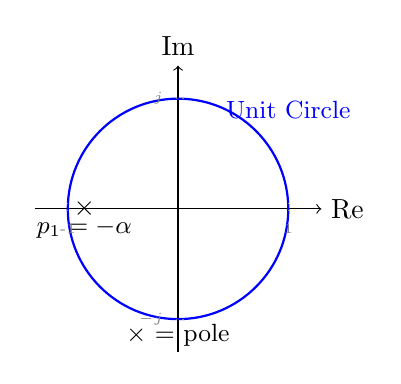
\begin{tikzpicture}[scale=1.4]
    % Draw axes
    \draw[->] (-1.3,0) -- (1.3,0) node[right] {Re};
    \draw[->] (0,-1.3) -- (0,1.3) node[above] {Im};
    
    % Draw unit circle
    \draw[thick, blue] (0,0) circle (1);
    
    % Add unit circle label
    \node[blue] at (1.0,0.9) {\small Unit Circle};
    
    % Mark pole on negative real axis inside unit circle
    \coordinate (p1) at (-0.85, 0);
    
    \node at (p1) {$\times$};
    
    % Label the pole
    \node[below] at (p1) {\small $p_1 = -\alpha$};
    
    % Add grid points for reference
    \draw[dotted, gray] (1,0.05) -- (1,-0.05) node[below] {\tiny 1};
    \draw[dotted, gray] (-1,0.05) -- (-1,-0.05) node[below] {\tiny -1};
    \draw[dotted, gray] (0.05,1) -- (-0.05,1) node[left] {\tiny $j$};
    \draw[dotted, gray] (0.05,-1) -- (-0.05,-1) node[left] {\tiny $-j$};
    
    % Legend
    \node at (0.0, -1.15) {\small $\times$ = pole};
    
\end{tikzpicture}
\end{center}

\vspace{0.3cm}

The pole is located at $z = -\alpha$ (where $ 0 < \alpha < 1$).

The corner frequency is then: $\omega_c = \pi - \arccos(\alpha)$

Assume $10 \omega_c$ is within the Nyquist frequency range ($10\omega_c < \pi$).

\vspace{0.5cm}

\begin{enumerate}
    \item \textbf{(10 points)} Based on the pole-zero plot above, 
    \begin{enumerate}[label=(\alph*)]
        \item \textbf{(6 points)} Sketch an approximation of the magnitude $|H(e^{j\omega})|$ and phase $\angle H(e^{j\omega})$ response.
        \item \textbf{(2 points)} In 1-2 sentences, explain how the pole location influences the shape of the magnitude and phase responses.
        \item \textbf{(2 points)} What type of filter does this system represent (e.g., low-pass, high-pass, band-pass, band-stop)?
    \end{enumerate}
\end{enumerate}

% \vspace{0.5cm}

% Magnitude Response Plot
% \textbf{Magnitude Response:}

\begin{center}
\begin{tikzpicture}[scale=0.75]
    % Axes
    \draw[->] (0,0) -- (8.5,0) node[right] {$\omega$ (log scale)};
    \draw[->] (0,0) -- (0,4) node[above] {$|H(e^{j\omega})|$ (dB)};
    
    % Tick marks on x-axis (log scale)
    \draw (2.33,0.05) -- (2.33,-0.05) node[below] {$0.1\omega_c$};
    \draw (4.66,0.05) -- (4.66,-0.05) node[below] {$\omega_c$};
    \draw (7,0.05) -- (7,-0.05) node[below] {$10\omega_c$};
    \draw (8.3,0.05) -- (8.3,-0.05) node[below] {$\pi$};
    
    % Solution plot (only if showresults is true)
    \ifthenelse{\boolean{showresults}}{
        % Tick marks on y-axis (dB) - only positive values
        \draw (0.05,1) -- (-0.05,1) node[left] {10};
        \draw (0.05,2) -- (-0.05,2) node[left] {20};
        \draw (0.05,3) -- (-0.05,3) node[left] {30};
        \draw (0.05,4) -- (-0.05,4) node[left] {40};
        
        % Draw flat region at low frequencies (0 dB/dec)
        \draw[thick, red] (0.5,0.5) -- (4.66,0.5);  % 0dB/dec (flat)
        
        % Draw +20dB/dec slope after corner freq
        \draw[thick, red] (4.66,0.5) -- (8.3,3.34);  % +20dB/dec slope extending to pi
        
        % Mark corner frequency
        \draw[dashed] (4.66,0) -- (4.66,0.5);
        \node[above] at (4.66,0.7) {\small Corner at $\omega_c$};
        
        % Add slope labels
        \node[above] at (2.5,0.8) {\small 0dB/dec};
        \node[above, rotate=20] at (6.5,2.0) {\small +20dB/dec};
    }{}
    
\end{tikzpicture}
\end{center}

% \vspace{0.5cm}

% Phase Response Plot
% \textbf{Phase Response:}

\begin{center}
\begin{tikzpicture}[scale=0.75]
    % Axes
    \draw[->] (0,0) -- (8.5,0) node[right] {$\omega$ (log scale)};
    \draw[->] (0,-3) -- (0,3) node[above] {$\angle H(e^{j\omega})$};
    
    % Tick marks on x-axis (log scale)
    \draw (2.33,0.05) -- (2.33,-0.05) node[below] {$0.1\omega_c$};
    \draw (4.66,0.05) -- (4.66,-0.05) node[below] {$\omega_c$};
    \draw (7,0.05) -- (7,-0.05) node[below] {$10\omega_c$};
    \draw (8.3,0.05) -- (8.3,-0.05) node[below] {$\pi$};
    
    % Tick marks on y-axis
    \draw (0.05,2) -- (-0.05,2) node[left] {$\pi$};
    \draw (0.05,1) -- (-0.05,1) node[left] {$\frac{\pi}{2}$};
    \draw (0.05,0) -- (-0.05,0) node[left] {0};
    \draw (0.05,-1) -- (-0.05,-1) node[left] {$-\frac{\pi}{2}$};
    \draw (0.05,-2) -- (-0.05,-2) node[left] {$-\pi$};
    
    % Solution plot (only if showresults is true)
    \ifthenelse{\boolean{showresults}}{
        % Plot curve - starts at 0, goes to -pi/2 at wc, approaches -pi at high freq
        % Pole at -alpha gives phase that goes from 0 to -pi
        \draw[thick, blue] plot[smooth, domain=0.5:8.3] 
            (\x, {-1.25*(1 + tanh(0.8*(\x-4.66)))});
        
        % Mark transition
        \draw[dashed] (4.66,-3) -- (4.66,3);
        \node[right] at (4.8,2.5) {\small Transition at $\omega_c$};
    }{}
    
\end{tikzpicture}
\end{center}

\vspace{1cm}

% Written solutions (only if showresults is true)
\ifthenelse{\boolean{showresults}}{
    \textbf{Solution:}
    
    
    \textbf{(b) Explanation:}
    
    At frequencies below $\omega_c$, the system has constant gain (0 dB/dec). Above $\omega_c$, the magnitude increases at $+20$dB/dec. The pole on the negative real axis causes the phase to transition from $0$ at low frequencies to $-\pi$ at high frequencies, with $-\pi/2$ phase at $\omega_c$.
    
    \vspace{0.5cm}
    
    \textbf{(c) Filter Type:}
    
    This system represents a \textbf{high-pass filter} because it attenuates low frequencies (constant, lower gain) and passes high frequencies with increasing gain. 
}{}



\end{document}